\documentclass[conference]{IEEEtran}
\IEEEoverridecommandlockouts
% The preceding line is only needed to identify funding in the first footnote. If that is unneeded, please comment it out.
\usepackage{cite}
\usepackage{minted}
\usepackage{amsmath,amssymb,amsfonts}
\usepackage{algorithmic}
\usepackage{graphicx}
\usepackage{textcomp}
\usepackage{xcolor}
\usepackage{lineno,hyperref}
\usepackage{todonotes}
\usepackage{multirow}

\usepackage{booktabs}
\def\BibTeX{{\rm B\kern-.05em{\sc i\kern-.025em b}\kern-.08em
    T\kern-.1667em\lower.7ex\hbox{E}\kern-.125emX}}

%%%%%%%%%%%%%%%%%%%%%%%%%%%%%%%%%%%%%%%%%%%%%%%%%%%%%%%%%%%
% Our import & commands

\newcommand{\TODO}[1]{{\color{magenta}{\bf #1}}}
\newcommand{\TBC}[1]{{\color{red}{\bf #1}}}

%%%%%%%%%%%%%%%%%%%%%%%%%%%%%%%%%%%%%%%%%%%%%%%%%%%%%%%%%%%

\begin{document}

%\title{Efficient Litter Detection in the Wild\\
%}
\title{Analisi e sperimentazione di tecniche \\ di Deep Learning per la ricerca di vulnerabilità \\ nel codice C, C++}

\author{
\IEEEauthorblockN{Elia Gaviraghi}
\IEEEauthorblockA{\textit{Approfondimento d'esame di Sicurezza Informatica, 2024}\\
Milano, Italy \\
% 0000-0002-7070-1545
}
% \and
% \IEEEauthorblockN{Elia Gaviraghi}
% \IEEEauthorblockA{\textit{Department of Informatics, Systems and Communication} \\
% \textit{University of Milano-Bicocca}\\
% Milano, Italy \\}
% \and
% \IEEEauthorblockN{Raimondo Schettini}
% \IEEEauthorblockA{\textit{Department of Informatics, Systems and Communication} \\
% \textit{University of Milano-Bicocca}\\
% Milano, Italy \\
% 0000-0001-7461-1451}
}

\maketitle

\begin{abstract}
Gli sviluppi recenti nel campo della sicurezza informatica si sono principalmente basati su tecniche di analisi statica e dinamica per individuare vulnerabilità nei sistemi software. Tuttavia, l'avvento del deep learning potrebbe aprire una promettente via per migliorare la scoperta di vulnerabilità. Questo articolo vuole comprendere ombre e luci di questo mondo tramite un approccio pratico, mettendo alla prova alcuni modelli comuni nell'ambito delle vulnerabilità CWE su codice C/C++.

Un'analisi dei dataset esistenti rivela significative sfide quali etichettature inconsistenti e ostacoli nell'usabilità degli stessi dati. Questi problemi limitano la capacità di utilizzo dei dati e pongono degli ostacoli nell'addestramento di modelli robusti.

Sintetizzando le intuizioni dei metodi tradizionali e integrando metodologie di deep learning, questo approfondimento mira a favorire una comprensione più approfondita del potenziale trasformativo del Deep Learning nella sicurezza informatica. Sono discusse analisi personali riguardo le limitazioni riscontrare e dilemmi riguardo la natura intrinseca dei dati riguardo le vulnerabilità.
\end{abstract}

\section{Introduzione}

Nell'era digitale odierna, la sicurezza informatica non può non essere considerata come una questione vitale per l'esistenza di un'azienda, un ente e di uno stato. Con l'aumento della complessità e della sofisticazione delle minacce informatiche, è necessario sviluppare metodi sempre più avanzati per rilevare e prevenire gli attacchi. In questo contesto, le tecniche di deep learning stanno emergendo come strumenti potenti per migliorare la nostra capacità di proteggere i sistemi informatici.

Questo approfondimento d'esame utilizza un approccio pratico per sperimentare l'applicazione di alcune architetture di deep learning presentate in \cite{russell2018automatedvulnerabilitydetectionsource} per l'analisi del codice sorgente C/C++, al fine di rilevare potenziali vulnerabilità sfruttando la famosa classificazione CWE\cite{cwe} per le vulnerabilità. Viene analizzato il dataset utilizzato dai modelli denominato VDISC, comprendendone potenzialità e limiti; gli esperimenti sono già stati parzialmente riprodotti in \cite{Ykartal2024}. 

Un nuovo un nuovo dataset è stato realizzato appositamente per l'approfondimento, ESED, estrapolando una costola del noto SARD prendendo solo il codice scritto nel linguaggio C/C++, permettendo di estendere l'analisi non solo ai modelli architetturali, ma concentrandosi anche sulle problematiche e le questioni dei dati in input a questi modelli di deep learning.

\textbf{L'obiettivo postosi dunque non è quello di competere per migliorare le performance riportate dagli autori sul paper o costruire un dataset di qualità maggiore che possa essere completo} - sarebbe quasi arrogante - ma si vuole andare a toccare con mano questo mondo in modo da far sorgere personalmente dilemmi e visioni riguardo potenzialità e limiti di queste soluzioni, oggigiorno applicate un po' ovunque, ragionando sui possibili vantaggi e svantaggi non sui massimi sistemi dello stato dell'arte, ma su dei casi reali affrontati.

Nel corso del paper, si descrivono in dettaglio i dataset utilizzati, il processo di costruzione del dataset ESED estrapolato da SARD, l'implementazione delle architetture di deep learning del paper e i risultati ottenuti. Infine, si discute le implicazioni dei nostri risultati nel quadro della sicurezza informatica per la sicurezza informatica e rifletteremo sulle potenziali applicazioni e sviluppi futuri di queste tecniche di deep learning.

\section{Datasets Disponibili}

Questa sezione non mira a essere una descrizione completa dello stato dell'arte, ma è necessaria per far comprendere il processo di realizzazione dell'approfondimento. 

Rispetto ad altri ambiti dove il deep learning risulta ormai essere la scelta principale a cui affidarsi, il campo della sicurezza informatica fatica ancora nell'uniformare la raccolta dei dati e la distribuzione di dataset che siano conosciuti, di ampie dimensioni e facilmente usufruibili, sia per una natura intrinseca del problema sia per una mancanza di standard comuni.

SARD \cite{209211}(Software Assurance Reference Dataset) risulta essere uno dei più famosi e promettenti dataset per fornire adeguate informazioni ai modelli di deep learning.  Curato dal NIST, SARD è una raccolta crescente di programmi organizzati singolarmente in test cases e raggruppati in test suite, etichettando la debolezza rilevata con la classificazione CWE; i test cases variano da piccoli programmi sintetici a grandi applicazioni.

VDISC (Vulnerability Detection in Source Code) è un dataset presentato in \cite{russell2018automatedvulnerabilitydetectionsource} che contiene la combinazione di più codici in linguaggi C/C++, in particolare viene utilizzata la \textit{juliet test suite 1.3} estratta da SARD, codice proveniente da Debian e dei non specificati repository su GitHub. Il dataset presentato viene descritto nel paper e risulta di immediato utilizzo, presentandosi in forma tabellare e fornendo il codice sorgente con una classificazione multi-etichetta binaria sulla base di diverse classi.

Il National Vulnerability Database (NVD), sempre gestito dal NIST, contiene anch'esso informazioni dettagliate su vulnerabilità software, ma in modo più sparpagliato e confuso: c'è una classificazione sia con CVE\cite{cve} che con CWE\cite{cwe} sia con uno score calcolato, ma l'accesso al codice relativo è alquanto difficoltoso.

CVEfixes \cite{bhandari2021:cvefixes} è un set di dati che contiene vulnerabilità con diversi linguaggi di programmazione provenienti dal NVD; l'estrapolazione di parte di questo dataset è disponibile anche su Kaggle e risulta di facile usabilità, visto che è disponibile un CSV con il codice sorgente e un'etichetta; peccato che quest'ultimo sia solamente un etichetta binaria per segnalare se il codice sia vulnerabile o no e non vi sia un'etichetta aggiuntiva riguardo la classificazione CVE/CWE, il che risulta insufficiente. L'estrapolazione dei dati provenienti invece dal dataset originale non è del tutto facilitata, anche se indubbiamente risulta più fattibile e valida per una ricerca nell'ambito

OSV (Open Source Vulnerability) - da non confondere con OSVDB, chiuso nel 2016 - è un progetto interessante che raccoglie e fornisce informazioni sulle vulnerabilità di solo software open-source. Le informazioni e il sito risultano user-friendly, ma il dato principale, ovvero il codice sorgente, non è facile da reperire, tenendo conto che si mettono insieme un grane quantitativo di risorse esterne non indifferenti.

Exploit Database (ExploitDB) è un altro database di exploit che ricorda inizialmente per struttura SARD. Tuttavia, non vengono definite delle suite scaricabili, quindi gli exploit sono scaricabili solo come test cases singoli; oltretutto, manca generalmente uno standard nella descrizione dell'exploit - a volte si trova un file JSON a descrizione, altre volte un file \texttt{.txt} che rassomiglia più a un file readme che a uno standard strutturato; in tutto ciò, non necessariamente viene presentato un riferimento a un codice sorgente.

Per chiudere la sezione, VulnDB è un software a uso commerciale enorme ma che non fornisce necessariamente il codice sorgente specifico per ogni vulnerabilità, oltre al fatto che, l'accesso al DB è disposto su diversi tier, da un piano gratuito fino a dei piani enterprise.

\section{Dataset utilizzati}
In questa sezione si descrivono più approfonditamente il dataset utilizzato VDISC e il dataset estrapolato da SARD realizzato per questo approfondimento, ESED.

\subsection{VDISC: analisi e obiettivi}

\subsubsection{Descrizione dataset}
VDISC è un dataset in forma tabellare con codice sorgente estrapolato prettamente da SARD e da altre fonti open-source; presenta uno split ufficiale in train, validation e test rispettivamente dell'80/10/10\%. 
La maggior parte del nostro set di dati è costruito con codice open source di cui non sono note le etichette, a differenza del codice proveniente da SARD. Le etichette allora sono state generate valutando tre approcci differenti: analisi statica, dinamica e valutazione dei tag sui messaggi di commit/segnalazione di bug.

L'analisi dinamica, per quanto possa essere efficace, è risultata estremamente dispendiosa in termini di risorse: l'utilizzo di essa su sole circa 400 funzioni ha richiesto una giornata intera di lavoro ai ricercatori, rendendone l'utilizzo irrealistico su una dataset con centinaia di migliaia di codici. Il tag delle commit è risultato troppo eterogeneo e di bassa qualità, non seguendo uno standard ma lasciando al singolo sviluppatore la composizione del messaggio, risultando inappropriato per il task richiesto. Infine, i ricercatori hanno dovuto optare per l'analisi statica incrociando i risultati di tre diversi tool: \textbf{Clang, Cppcheck e il noto Flawfinder, i quali hanno generato degli output che sono poi stati interpretati da un team di persone umani}, ottenendo 390 tipi diversi di CWE, su cui è stato fatto un sotto campionamento a 149 vulnerabilità dal team di ricercatori. 

\textbf{Una riflessione personale è sorta allora riguardo queste etichette}: etichettando i dati incrociando gli output dei tool di analisi statica, i dati stessi ne ereditano gli stessi limiti, a meno di un ulteriore controllo umano approfondito ed esperto, ma infattibile su larga scala. Ci si può allora domandare dove possa risiedere il vantaggio di addestrare un modello di deep learning, il quale comporta ingenti risorse hardware e un non indifferente tempo di sviluppo, \textbf{se la sua conoscenza deriva da tool già esistenti di analisi statica?} 

La speranza, a parere personale, risiede nel riuscire a ottenere non uno strumento specifico, bensì ottenere un modello che possa racchiudere tutte le potenzialità di questi - prendi 1, ottieni 3.

Chiunque tratti l'arte del deep learning tuttavia, è consapevole che per raggiungere determinate performance su un vasto numero di classi - per esempio 149, quelle selezionate dal team di ricerca - il quantitativo di dati, oltre alla loro qualità, deve essere assai altissimo per permettere al modello di riconoscere le classi e generalizzare su dati mai visti. Difatti, anche se non esplicitato nella ricerca, il dataset prevede solo 4 vulnerabilità CWE specifiche, mentre è stata creata una quinta etichetta per accorpare tutte le altre CWE presenti, andando a confermare l'infattibilità attuale della considerazione precedente.
%
\begin{figure}[h]
    \centering
    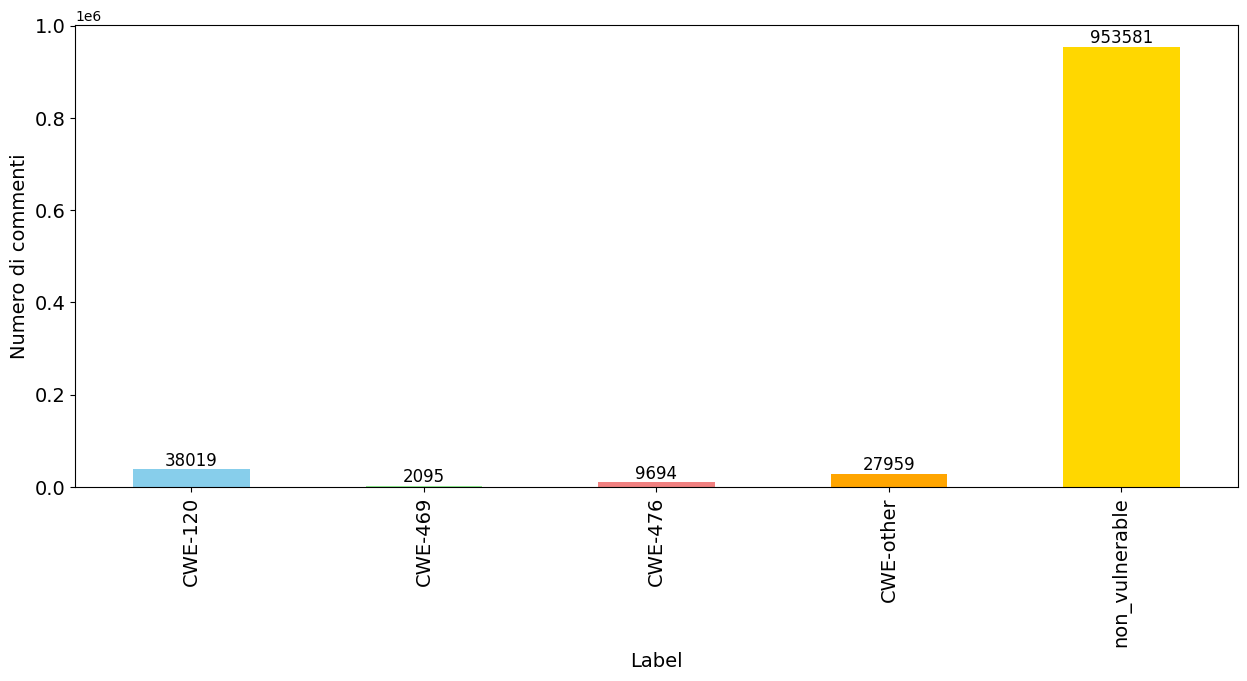
\includegraphics[width=\columnwidth]{images/VDISC/OSF-distribution.png}
    \caption{Distribuzione delle etichette all'interno del dataset}
    \label{fig:distribuzione-etichette}
\end{figure}
%
Riguardo la qualità dei dati, si pone un ulteriore interrogativo: il dataset risulta alquanto sbilanciato \ref{fig:distribuzione-etichette} con la maggior parte del codice presente  la maggior parte del codice come non vulnerabile: ne conseguirà uno sbilanciamento nelle performance e un'attenta analisi delle metriche di valutazione per non incappare in false speranze, avendo praticamente solo 64.890 esempi di codice con vulnerabilità

Inoltre, sebbene il dataset ammetta più etichette binarie attive contemporaneamente, la maggior parte del codice etichettato come vulnerabile risulta avere solamente un'etichetta attiva \ref{fig:distribuzione-tag}, ponendo un secondo sbilanciamento aggiuntivo.
\begin{figure}
    \centering
    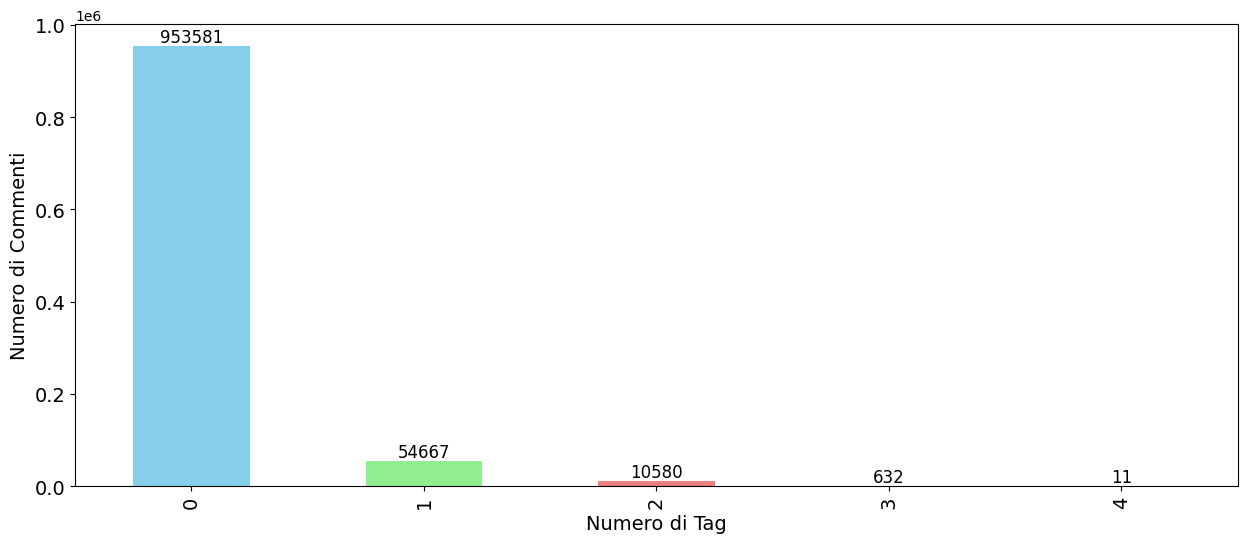
\includegraphics[width=\columnwidth]{images/VDISC/OSF-num-tag.png}
    \caption{Distribuzione del numero di esempi nel dataset in base al numero di label binarie attive}
    \label{fig:distribuzione-tag}
\end{figure}
%
Lo sbilanciamento principale risulta comunque essere il primo\ref{fig:distribuzione-etichette}, e la riflessione principale che deve essere fatta prima di manipolare i dati riguarda la realtà dello scenario: se questo sbilanciamento non risulta essere una mancanza del dataset in questione, ma una rappresentazione della realtà (ovvero nella maggior parte del codice io non avrò vulnerabilità), allora ha senso mantenere tale proprietà. Questa riflessione non trova però risposte certe, lasciando ulteriori conclusioni ad analisi successive

    
\subsubsection{Analisi e obiettivi su VDISC}
L'obiettivo posto non è quello di superare le performance ottenute dagli autori \cite{russell2018automatedvulnerabilitydetectionsource}, ma di sperimentare e comprendere potenzialità e limiti di questo dataset e i modelli di ML. Si è inoltre compreso che i risultati riportati nella ricerca non sono del tutto riproducibili, in quanto risultano mancanti varie informazioni cruciali, tra cui: 
\begin{itemize}
    \item Non sono disponibili nel dettaglio le architetture utilizzando, mostrando solo quanto realizzato a un alto/medio livello e non avendo accesso al valore di alcuni parametri, come per esempio del \texttt{maxpooling} nella la CNN.
    %
    \item Non sono resi noti i valori decisivi per il processo di tokenization; vengono riportato dei parametri generici, come la lunghezza esatta delle sequenze che viene indicata con un valore generico tra $10 < l < 500$.
    %
    \item Non viene riportato esattamente come gli autori hanno interpretato il problema, ovvero di come i vari modelli effettuano la predizione in termini di numeri e di classi, lasciando aperta la questione a singole interpretazioni. 
    Di primo impatto, sembrerebbe logico implementare in tutti i modelli come output un singolo layer \texttt{dense} con un numero di unità corrispondente al numero di etichette presenti nel dataset (dunque 5) e con funzione di attivazione \textbf{sigmoide}, interpretando il problema come una classificazione multi-etichetta binaria, monitorando l'andamento del training tramite la \textit{loss function} conosciuta come \textit{binary cross entropy}. Le uniche menzioni riguardano la funzione di attivazione usata in dei ipotetici layer di output, che è la \textit{softmax}, e soprattutto menzionano di aver utilizzato la \textit{cross entropy} come \textit{loss function}, il che appare alquanto particolare.
    %
    \item Gli autori non riportano il valore del seed e altri valori utili per la riproducibilità dei risultati, per cui è quasi impossibile ottenere i medesimi risultati.
\end{itemize}


\subsubsection{Esperimenti pregressi}

Come punto di partenza, si è fatto poi riferimento a questo repository\cite{Ykartal2024} disponibile su GitHub, in cui l'autore ha cercato di riprodurre alcune delle architetture utilizzate nel paper \cite{russell2018automatedvulnerabilitydetectionsource}. 

A livello architetturale è stata fatta un'interpretazione particolare: si è scelto di utilizzare una codifica one-hot-encoding con un layer di output per ogni label, quindi in totale ottenendone 5, e disponendo la funzione di attivazione \textit{softmax} per ognuno di questi layer. Si affronta così il problema come multi classe per ogni singola etichetta, e ciò va in contrasto con la generica \textit{cross entropy} utilizzata nel paper, visto che si fa utilizzo della \textit{categorical cross entropy}. Inoltre, bisognerà prestare molta attenzione ai risultati ottenuti durante il training con questo codice, visto che la matrice di confusione risulterà inversa e le metriche di \textit{precision} e \textit{recall} risulteranno alte in apparenza per una interpretazione logicamente errata.

\subsection{Da Sard a ESED}

In questa sezione si descrive l'analisi del dataset SARD e l'estrapolazione dei dati per la realizzazione di un dataset nel contesto di questo approfondimento.

\subsubsection{SARD}
SARD è un vasto database curato dal NIST, in cui i codici presenti sono scritti nei linguaggi C/C++, Java, PHP e C\# e vanno a coprire oltre 150 classi CWE di vulnerabilità. SARD offre due cose interessanti: delle test suites scaricabili, come raccolta di più test cases, in cui è contenuta sia l'etichettamento della vulnerabilità che un codice sorgente affetto alla stessa vulnerabilità. Si presenta ora un esempio di test case in linguaggio C
\begin{minted}{c}
int main() {
    void(*funcPtr)(void);
}
\end{minted}
come anticipato, l'etichettamento avviene seguendo il CWE, e in questo caso la vulnerabilità viene etichettata come \textit{CWE-563: Assignment to Variable without Use}. Inoltre, nel file \texttt{manifest.serif} in ogni test cases si fa riferimento al codice sorgente (scaricato in locale insieme al test cases) e a un sottoinsieme specifico del codice che causa la vulnerabilità. \\
Nonostante questo grande potenziale, l'utilizzo dei dati raccolti per i con modelli di deep learning non è immediato: bisogna scaricare le test suite in locale, estrarle (il che comporta una notevole perdita di tempo) e generare il codice in locale per creare un dataframe con le quattro informazioni principali:
\begin{itemize}
    \item ID del test cases
    %
    \item Il codice sorgente
    %
    \item La specifica regione di codice che causa la vulnerabilità
    %
    \item L'etichettamento CWE del test cases
\end{itemize}
L'obiettivo è quello di creare una semplice tabella con cui poi andare ad affrontare un problema di processamento del testo NLP, premettendo di valutare la qualità ei dati presenti. Uno dei punti nevralgici che riguarda SARD consiste nel fatto che ogni test cases viene etichettato con una singola CWE: non si considerano possibili codici con più vulnerabilità contemporanee, e ciò può essere sii da un lato una semplificazione svantaggiosa, ma al contempo una restrizione troppo ampia della realtà, visto che un codice potrebbe essere affetto a più vulnerabilità (CWE) diversi; inoltre, risulterebbe necessario integrare con altrettanti esempi di codice che siano non affetti da vulnerabilità, al fine di poter un dataset realistico.


\subsubsection{Costruzione ESED}
L'Extract Sard Easy Dataset (ESED) è un \textbf{dataset realizzato appositamente per questo approfondimento d'esame, estrapolando una parte delle test suite scritte in codice C/C++ disponibili su SARD}. La necessità di costruire questo dataset è sorta per andare a toccare direttamente le potenzialità e i problemi derivanti di uno dei dataset potenzialmente più interessanti nel panorama attuale, comprendendo se esso potesse condividere i medesimi limiti emersi dal dataset VDISC descritti nella sezione successiva.

Un grande ostacolo per la costruzione di dataset di grandi dimensioni riguarda le personali capacità hardware: per quanto possa sembrare banale, trattare directory sii di dimensioni sull'ordine di qualche Gigabyte, ma composte da un'enormità i file di piccole dimensioni, porta a continui crash, rallentamenti e disagi nei tempi di esecuzione, nonostante la logica alquanto semplice per la realizzazione.

A livello tecnico, è stata prima fatta un'esplorazione di fattibilità per verificare la reperibilità delle informazioni necessarie, ovvero del codice sorgente e di un etichetta valida (CWE oppure CVE). È stata trovata risposta affermativa nel file \texttt{manifest.serif} di ogni sottodirectory per la rispettiva test-suite: questo contiene le informazioni sul linguaggio utilizzato per il check di quanto desiderato, la classificazione CWE della vulnerabilità individuata, il path del file sorgente interessato e in aggiunta, facoltativamente, anche la regione di codice specifica che causa la vulnerabilità.

Per la costruzione del dataset si sono scaricate le principali test suites disponibili su SARD\cite{209211}, tra cui le principali sono la \textit{Juliet C/C++ 1.3.1 with extra support} con più i 60.000 test cases e la \textit{IARPA STONESOUP Phase 3 - Test Cases}, con più di 7.000 report di vulnerabilità. Altre suite minori sono state utilizzate, e in alcuni casi sono risultate particolarmente utili per rafforzare la rappresentazione di specifiche classi CWE, come la test suite \textit{A Taxonomy of Buffer Overflows}. 

Una volta finito il lungo processo di estrazione dei dati, si sono accorpati i vari dataframe ottenute dalle diverse test suites, ottenendo un file \texttt{CSV} con 73.476 esempi e 189 classi CWE diverse. 

\begin{figure}[h]
    \centering
    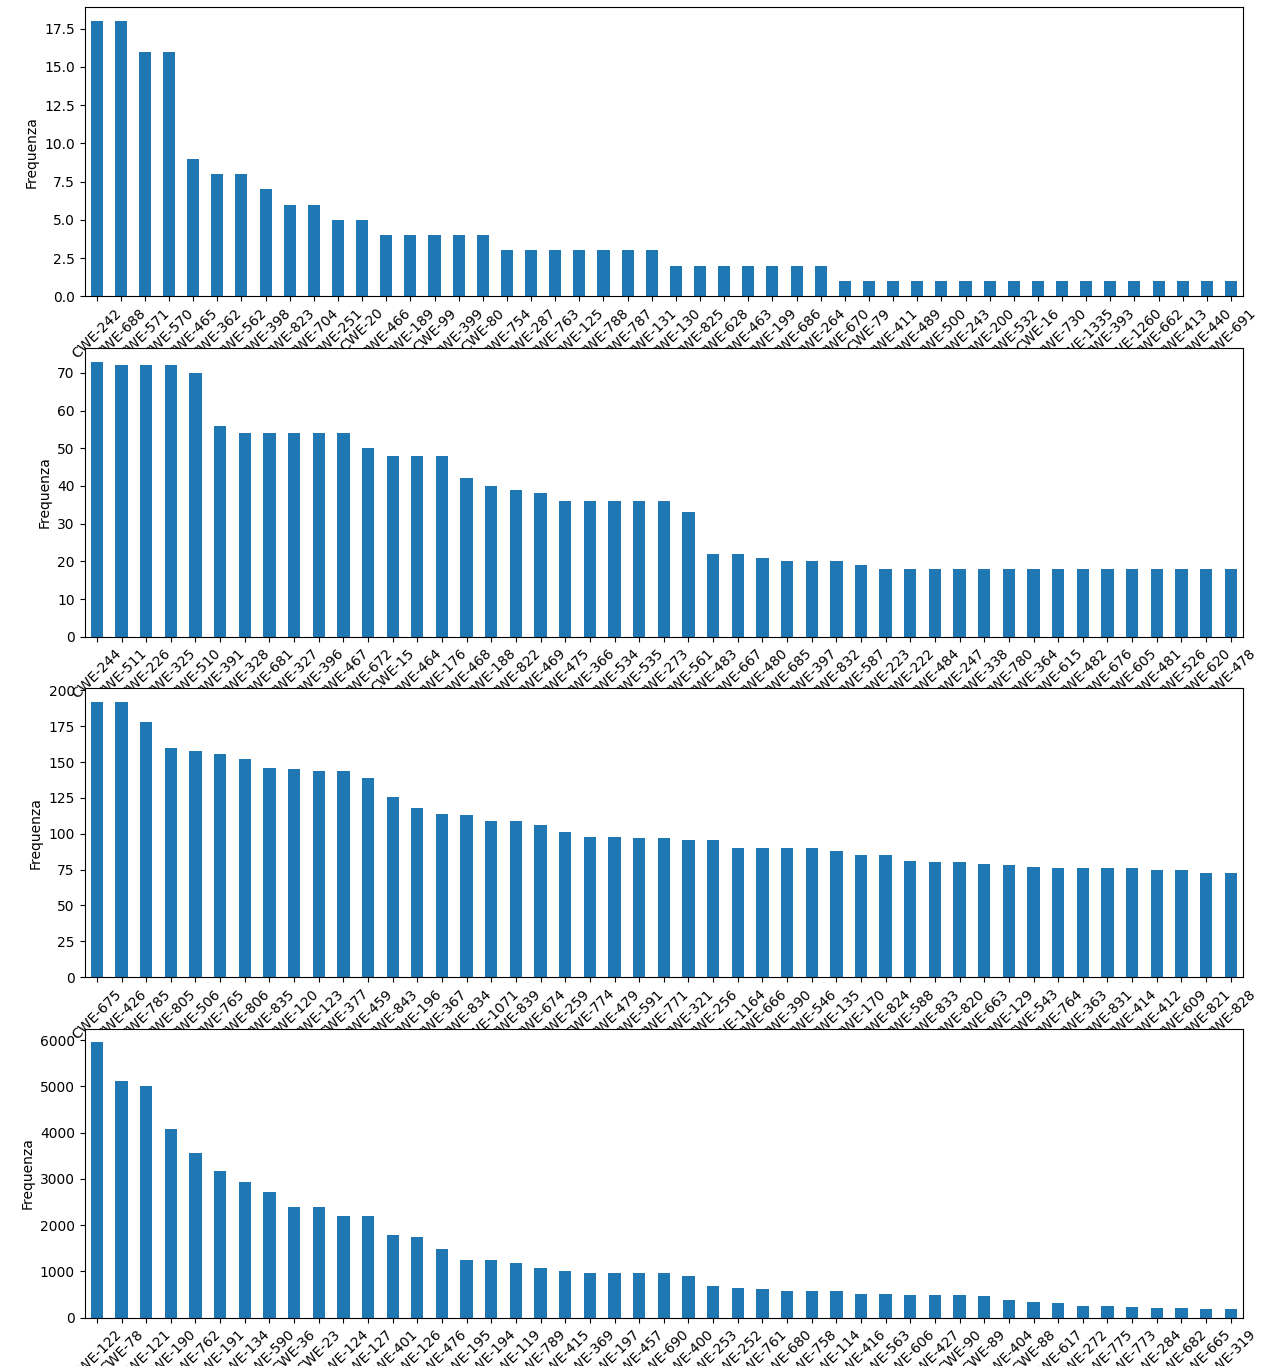
\includegraphics[width=\columnwidth]{images/ESED/SARD_GENERATE_label_distribution.png}
    \caption{Rappresentanza per ogni classe CWE all'interno del dataset ESED realizzato}
    \label{fig:class-on-esed}
\end{figure}

Questi dati, seppur possano sembrare di grandi dimensioni, non costituiscono un dataset così ampio per i modelli di deep learning; nello specifico, il numero di esempi disponibili per ogni classe non è uniforme, portando indubbiamente allo scarto di alcune classi raccolte; si noti però che sono circa 25 le classi che presentano più di 1.000 esempi, anche se i numeri devono poi far spazio a ulteriore analisi di qualità dei dati relativi al problema.


Un problema maggiore si riscontra sulle lunghezze delle stringhe che rappresentano il codice sorgente (\texttt{source}) e la porzione di codice problematico (\texttt{region}). 

\begin{figure}[h]
    \centering
    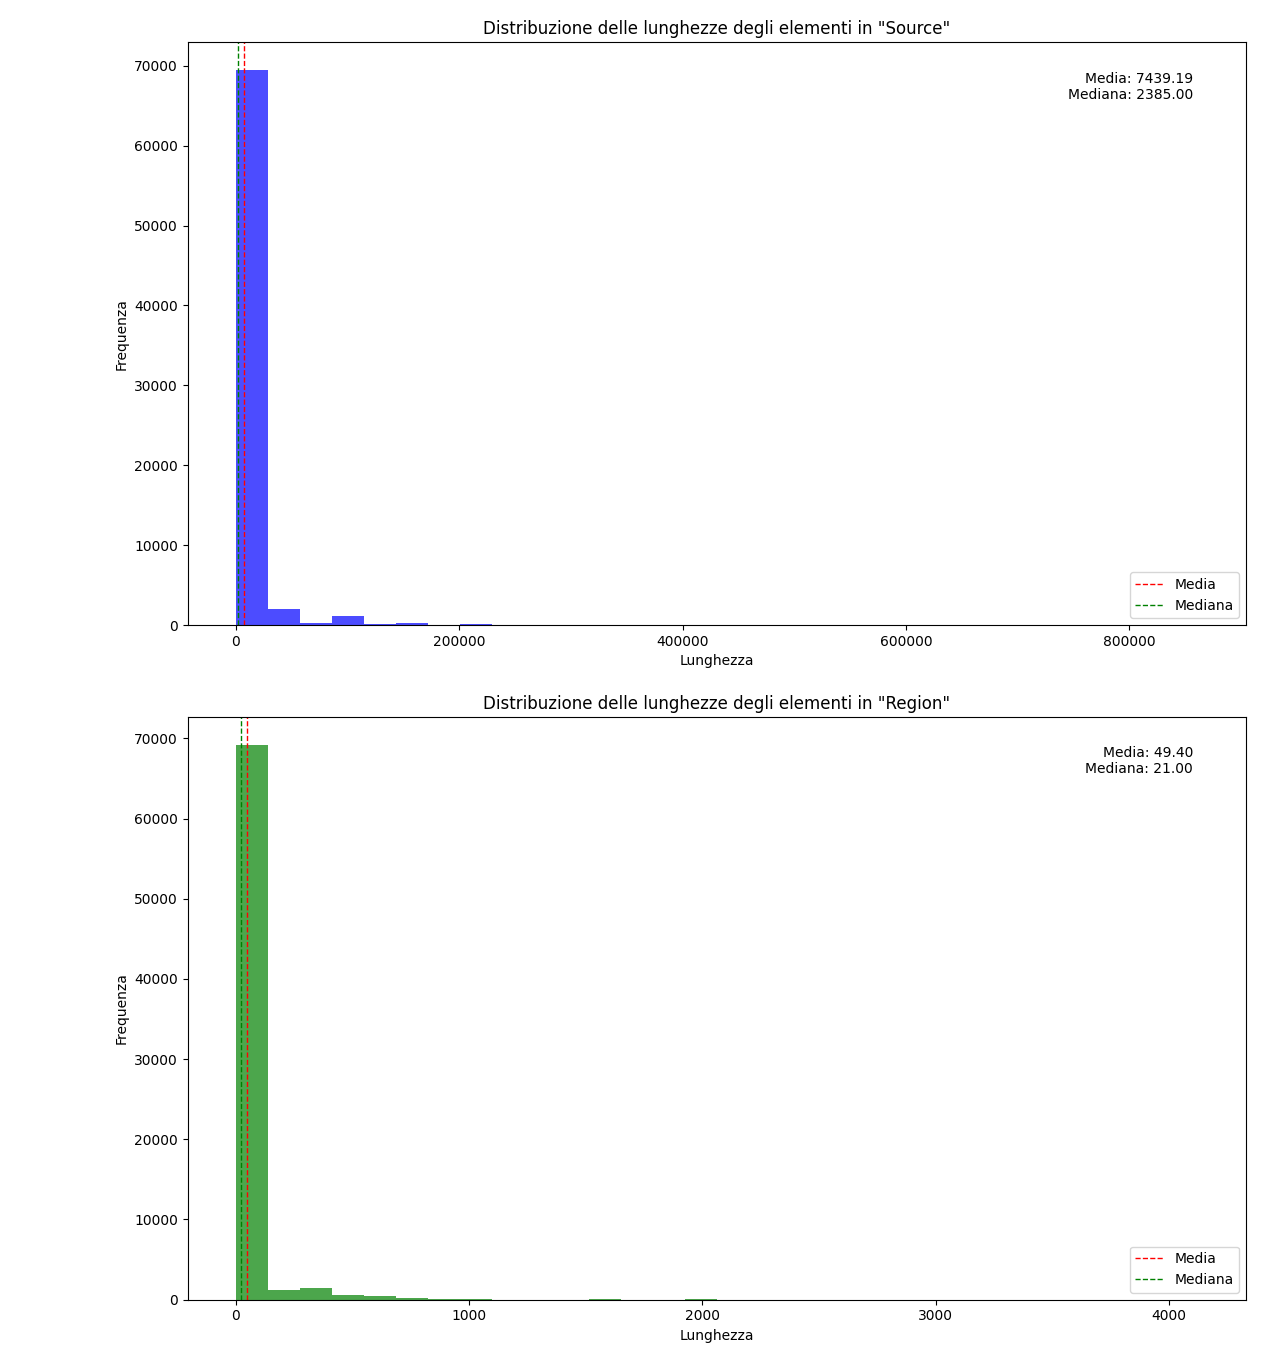
\includegraphics[width=\columnwidth]{images/ESED/SARD_GENERATE_lenght_source_region.png}
    \caption{Distribuzione delle lunghezze del codice presente in \texttt{source} e in \texttt{region}}
    \label{fig:length-source-region}
\end{figure}

Premesso che non sempre le test suites indicano le linee di codice problematico, portando a avere dei \texttt{NaN} nella colonna, la lunghezza delle stringhe in quest'ultima colonna è sicuramente più abbordabile della lunghezza media e mediana dei codici nel campo source. Ogni modello di deep learning, anche il più avanzato, presenta dei limiti più o meno grandi nell'input che riceve: \textbf{non si tratta solo di risorse hardware mancanti}- sequenze più lunghe richiede un hardware maggiore - ma anche di \textbf{comporre un'adeguata architettura in grado di catturare le informazioni rilevanti su un input di dimensione maggiore}. Può, tuttavia, l'informazione parziale riguardo della regione del codice vulnerabile essere sufficiente per la rilevazione di features per le future predizioni? Oppure è necessario non scendere a compromessi e utilizzare tutto il codice sorgente disponibile?

\section{Experimental results}

Questa sezione descrive gli esperimenti effettuati sui dataset VDISC ed ESED, al fine della riproduzione e l'esplorazione di modifiche alle architetture e al dataset presente.

\subsection{Experimental setup}
In ambo i casi, le risorse hardware utilizzate sono limitate: per l'estrapolazione dei dati da SARD è stato utilizzato l'ambiente locale su un comune laptop (i5 8250u, 24GB RAM, NVidia GTX 940mx); per l'addestramento delle architetture di deep learning e tutto il restante codice, è stato utilizzato Google Colab nella sua versione free, con GPU T4 che dispone di 15GB vRAM e 3 ore di sessione giornaliere. La mancanza di adeguate risorse hardware in locale ha rallentato di molto l'arrivo alla sperimentazione su Colab.

\subsection{Risultati VDISC}

Si è cercato di riprodurre i risultati ottenuti in \cite{Ykartal2024}, comprendendo le varie operazioni preliminari prima di arrivare alla tokenization e alla realizzazione del modello. 

Il primo esperimento fatto riguarda la costruzione della CNN così come viene presentata sul repository di GitHub, il quale mira a riprodurre quella presentata nel paper originario. L'architettura della CNN è un po' obsoleta: si mira ad avere un solo layer convoluzionale grande, anziché aumentare la profondità con layer più snelli, e si tratta il problema come multi-classe a livello di singolo output. Non si approfondisce oltre, non essendo un approfondimento di deep learnging, ma si riporta che, rispetto all'esperimento originale, si è dovuta snellire la fase di tokenization diminuendo la lunghezze delle sequenze, a causa del limite di RAM disponibile. I risultati ottenuti con questo esperimento non sono molto buoni: il modello fatica molto a rilevare i casi di vulnerabilità, molto probabilmente a causa del forte sbilanciamento; per l'etichetta CWE-469 il modello non riesce a rilevare nemmeno una vulnerabilità.

\begin{figure}[h]
    \centering
    \resizebox{\columnwidth}{!}{
    \begin{tabular}{cc}
        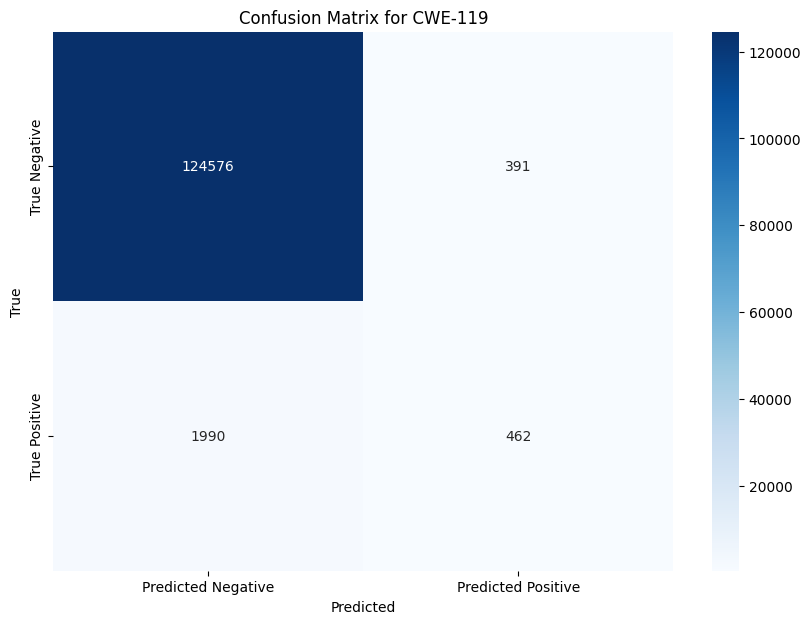
\includegraphics[width=0.5\textwidth]{images/VDISC/First_CNN/CWE-119-MTRX.png} & 
        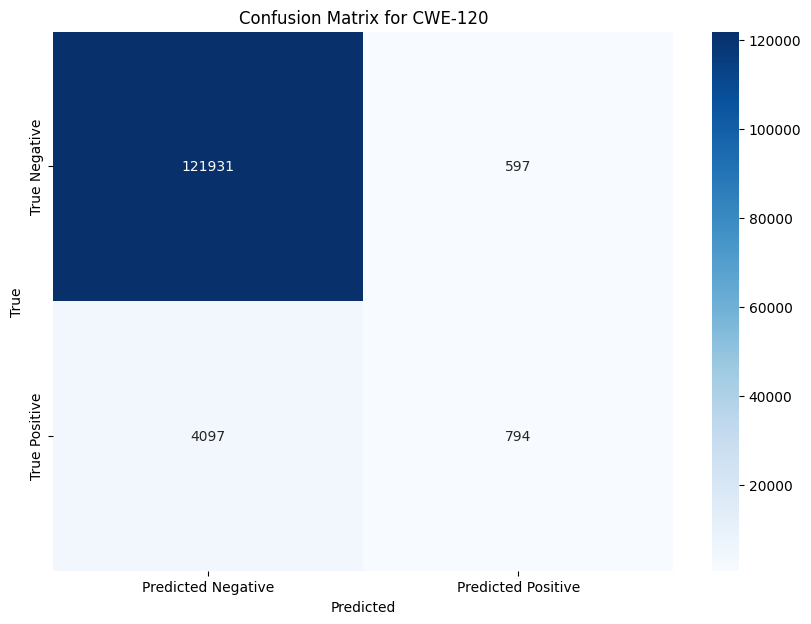
\includegraphics[width=0.5\textwidth]{images/VDISC/First_CNN/CWE-120-MTRX.png} \\ 
        
        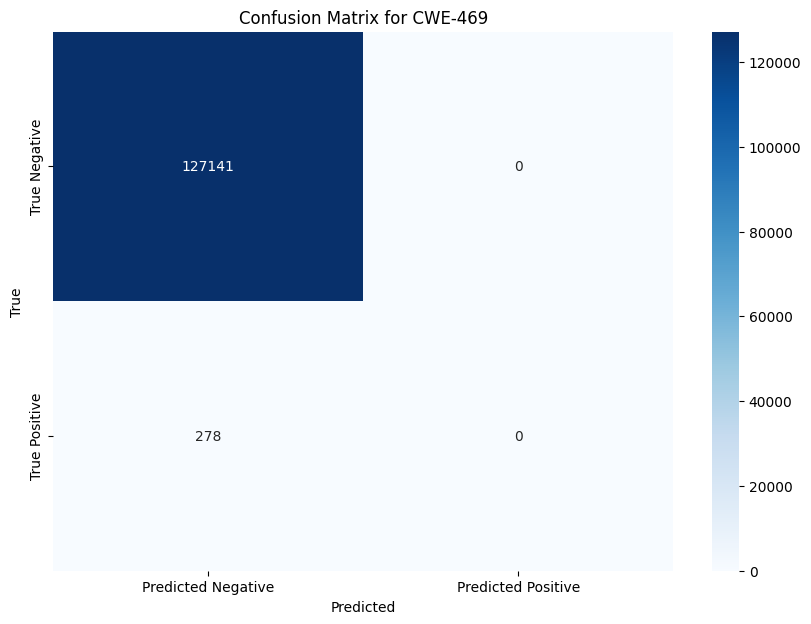
\includegraphics[width=0.5\textwidth]{images/VDISC/First_CNN/CWE-469-MTRX.png} &
        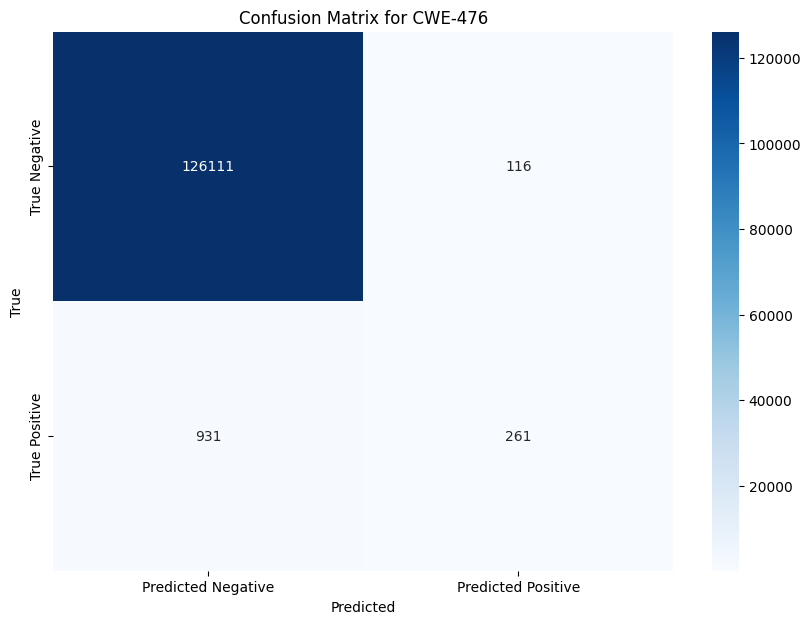
\includegraphics[width=0.5\textwidth]{images/VDISC/First_CNN/CWE-476-MTRX.png} \\
     \end{tabular}}
    \caption{Matrici di confusione relative al primo esperimento}
    \label{fig:confidence_effect}
\end{figure}

Durante il training bisogna considerare che la matrice di confusione è inversa nella interpretazione che interessa (i casi di vulnerabilità sono i \textit{True Positive}), dunque le metriche di precision e recall sono fuorvianti durante il training. Non ci si deve far ingannare anche dall'accuracy alta, perché avendo il dataset sbilanciato, se costruissimo un modello che risponde sempre 0 (quindi etichetta tutto come non vulnerabile) essa sarebbe comunque alta.

Il secondo esperimento compiuto riguarda l'utilizzo della precedente CNN, ma applicando la tecnica di undersampling alla "classe logica" dei non vulnerabili, ovvero mantenendo solo un rapporto di 1:4 tra vulnerabili:non-vulnerabili (almeno un etichetta a 1 vs tutte le etichette a 0). Anche questo esperimento non ha avuto esiti sperati.

Con un terzo esperimento si è deciso di cambiare l'architettura proposta, modificando l'output con un solo layer e interpretando il problema come un \textit{multi-label binary classification}: ora durante il training si possono visualizzare le metriche corrette e monitorare meglio l'andamento della situazione. Al fine di implementare i pesi delle varie classi, è stata creata una sesta etichetta denominata: "not\_vulnerable" per rappresentare tutti quegli esempi non vulnerabili. 

\begin{figure}[H]
    \centering
    \resizebox{\columnwidth}{!}{
    \begin{tabular}{cc}        
        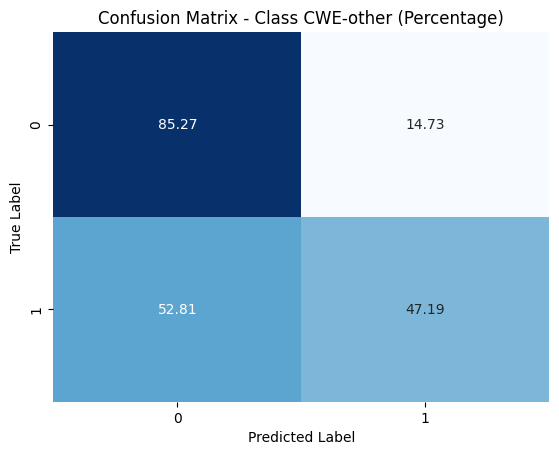
\includegraphics[width=0.5\textwidth]{images/VDISC/Third_CNN/CWE-other.png} &
        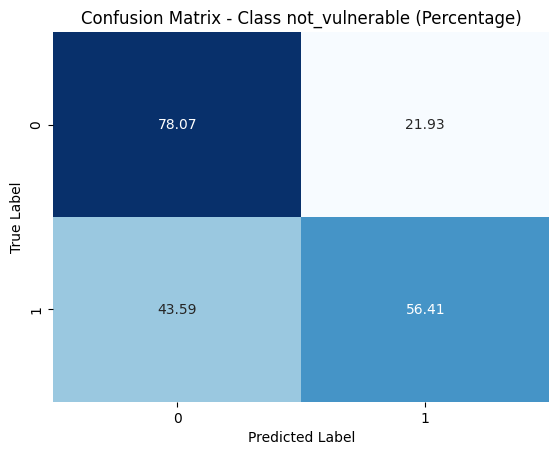
\includegraphics[width=0.5\textwidth]{images/VDISC/Third_CNN/not-vulnerable.png} \\
     \end{tabular}}
    \caption{Le uniche due matrici di confusioni rilevanti del terzo risultato}
    \label{fig:confidence_effect}
\end{figure}

I risultati anche qui non sono per nulla ottimali, ottenendo mediocri performance in precision-recall nei non vulnerabili e nella CWE-other, che raccoglie diverse vulnerabilità CWE, mentre sulle restanti classi restanti viene predetto come tutto non vulnerabile - ciò suggerirebbe magari che si possa ragionare su un problema di singola etichetta binaria sulla vulnerabilità, ma uno strumento del genere non servirebbe, a meno di essere utilizzato in un più dispendioso processo che prevede due o più classificatori.

Un quarto esperimento replica il precedente esperimento effettuando un undersampling sempre sui non vulnerabili, ma i risultati restano ancora scarsi.

\begin{table}[H]
    \begin{tabular}{rcccc}
        \multicolumn{1}{l}{} & \textbf{Precision} & \textbf{Recall} & \textbf{F1-score} & \textbf{Support} \\
        CWE-119         & 0.03 & 0.07 & 0.04 & 2452   \\
        CWE-120         & 0.06 & 0.21 & 0.09 & 4891   \\
        CWE-469         & 0.01 & 0.05 & 0.02 & 278    \\
        CWE-476         & 0.02 & 0.11 & 0.03 & 1192   \\
        CWE-other       & 0.04 & 0.14 & 0.06 & 3490   \\
        not\_vulnerable & 0.95 & 0.63 & 0.76 & 119166 \\
        micro avg       & 0.61 & 0.59 & 0.60 & 131469 \\
        macro avg       & 0.18 & 0.20 & 0.17 & 131469 \\
        weighted avg    & 0.86 & 0.59 & 0.69 & 131469 \\
        samples avg     & 0.60 & 0.60 & 0.60 & 131469
    \end{tabular}
    \caption{Risultato sul test set VDISC con la CNN del quarto esperimento}
\end{table}
%
La lunghezza delle sequenze è stata alzata a 500, il massimo valore del range indicato dagli autori, grazie alla diminuzione dei dati in input eseguendo un undersampling sul training set con rapporto 1:2 vulnerabili-non vulnerabili. Il problema è che questo sbilanciamento persiste nel validation e test set, dove non si dovrebbe mai agire con queste tecniche.

Il quinto e ultimo esperimento vede il cambio di architettura, nella speranza di poter migliorare la situazione in extremis; viene introdotta una LSTM molto leggera al posto della CNN; la realizzazione di questa architettura è stata possibile solo grazie all'esperienza maturata sul dataset ESED descritto nella sezione successiva.  Si è mantenuto l'assetto del quarto esperimento, quindi introducendo la classe per i non vulnerabili e e l'undersampling con rapporto 1:2 sul training set. Oltre all'architettura in sé, si sono "aggiustati" alcuni parametri in comune con la CNN, come la dimensione dell'output dell'embedding layer: nella CNN del paper si utilizzava un valore di 13, alquanto inusuale, ed è stato aumentato a 32 - comunque basso rispetto al comune, per evitare di incappare nell'overfitting. Inizialmente l'andamento del training sembrava finalmente più promettente rispetto alle prove precedenti\ref{fig:train-RNN-VDISC}
%
\begin{figure}[h]
    \centering
    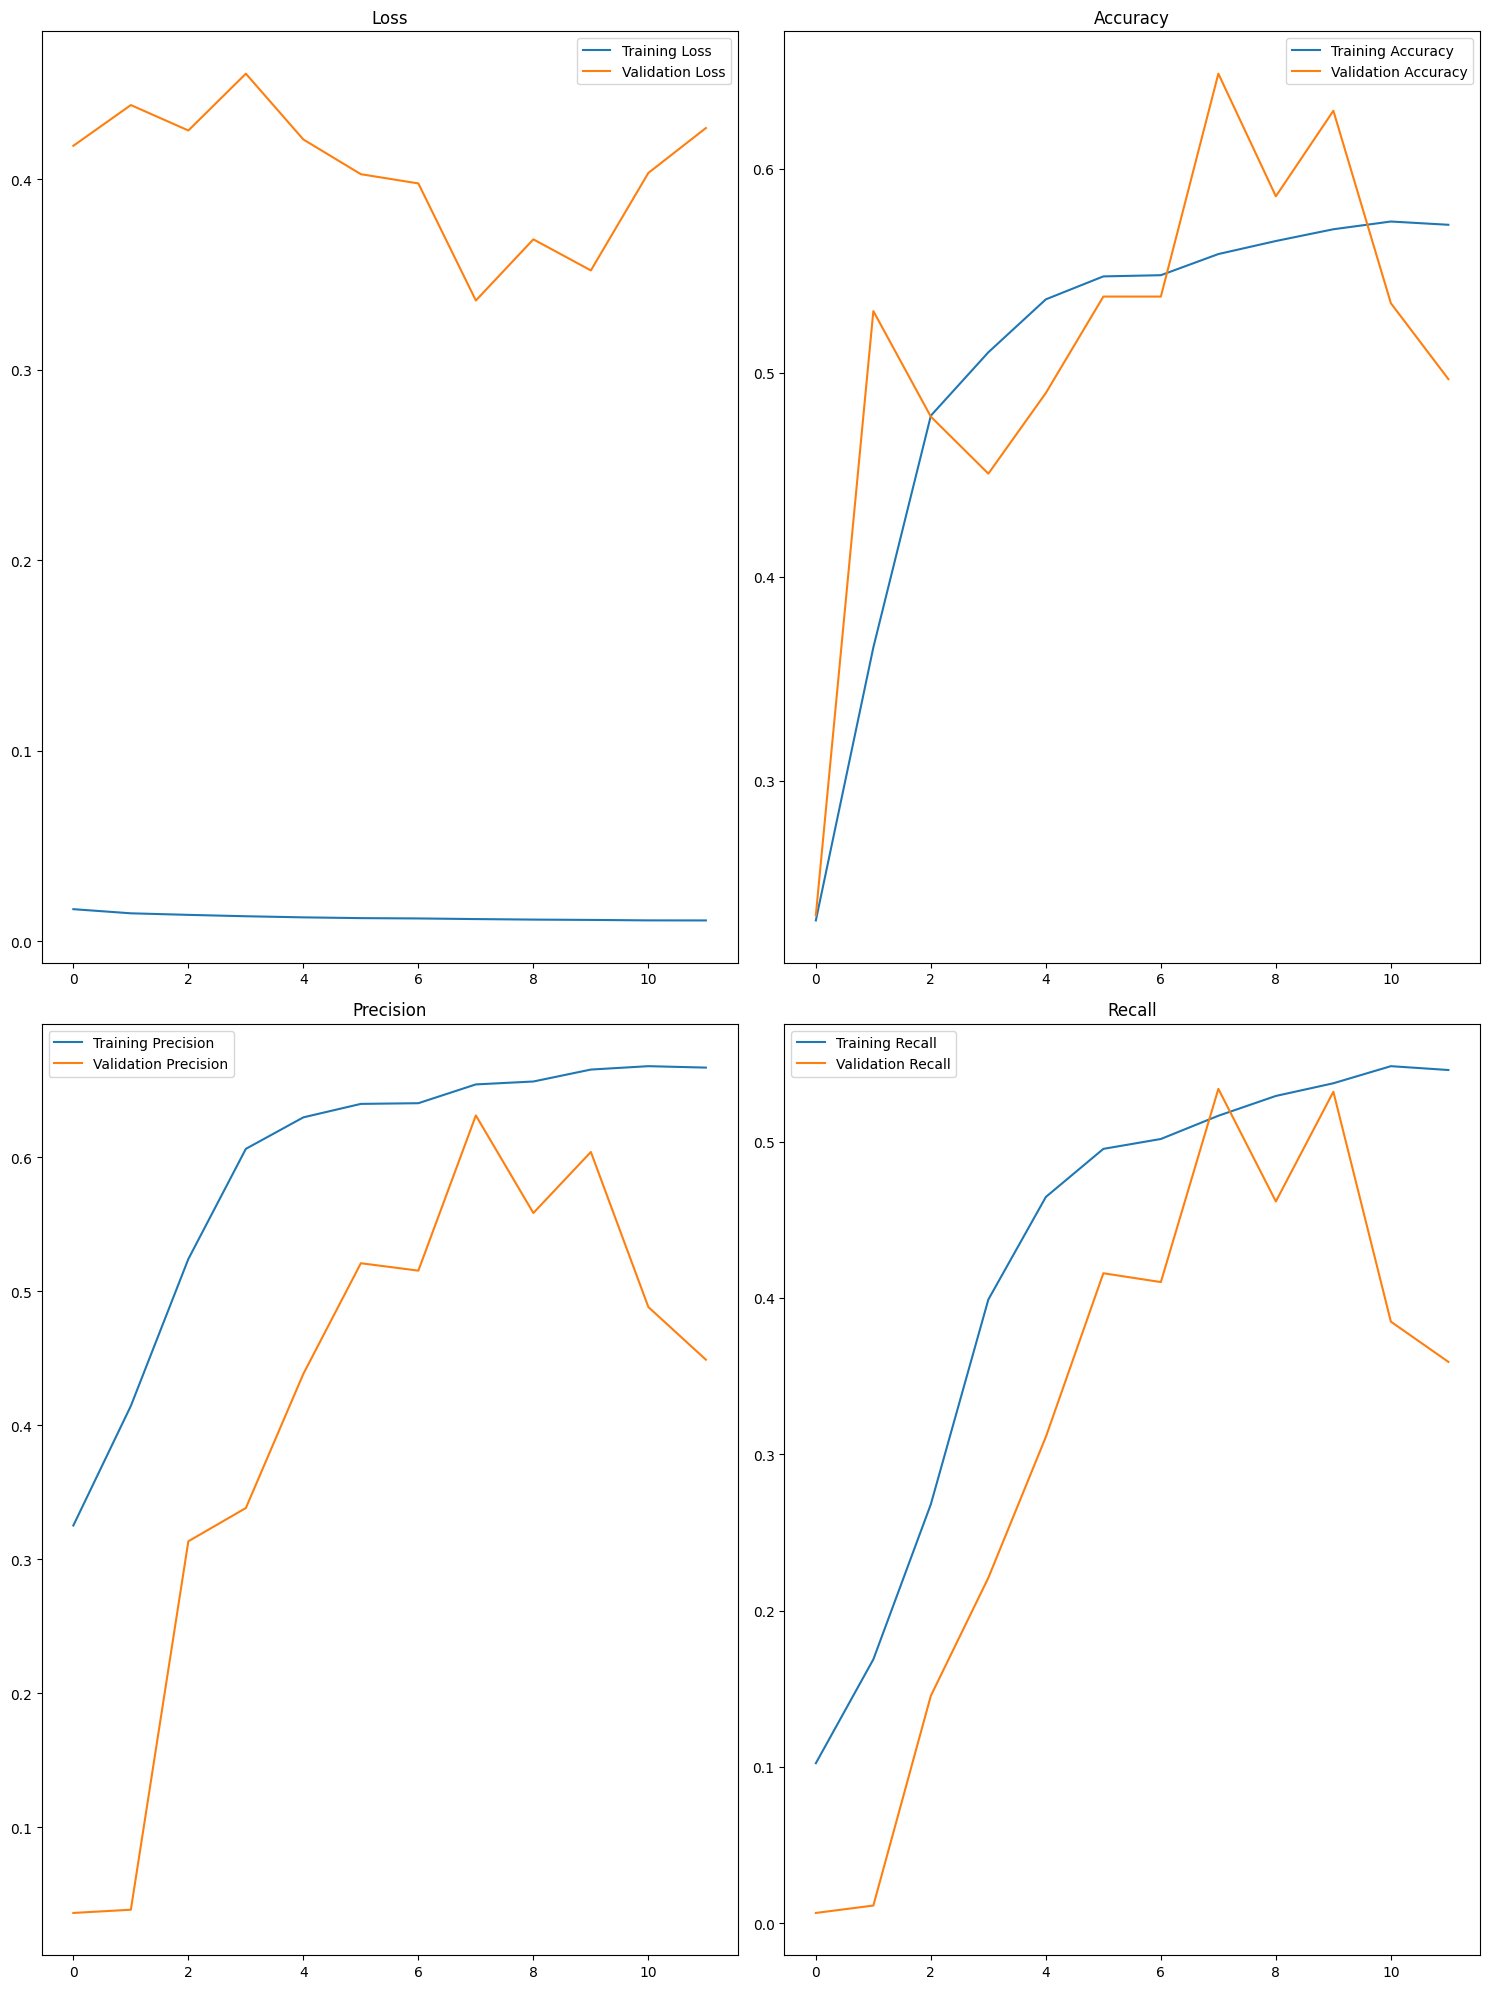
\includegraphics[width=\columnwidth]{images/VDISC/last_RNN/training_val.png}
    \caption{L'andamento del training su train e validation set con la RNN sul dataset VDISC}
    \label{fig:train-RNN-VDISC}
\end{figure}
%
Purtroppo quanto ottenuto non è quello sperato: i risultati sul test set non è stato per nulla quello sperato, mantenendo la situazione analoga alle precedenti, per quanto leggermente migliore.
%
\begin{table}[h]
    \begin{tabular}{rcccc}
        \multicolumn{1}{l}{} & \textbf{Precision} & \textbf{Recall} & \textbf{F1-score} & \textbf{Support} \\
        CWE-119              & 0.02               & 0.06            & 0.03              & 2452             \\
        CWE-120              & 0.06               & 0.23            & 0.09              & 4891             \\
        CWE-469              & 0.00               & 0.00            & 0.00              & 278              \\
        CWE-476              & 0.02               & 0.09            & 0.03              & 1192             \\
        CWE-other            & 0.04               & 0.05            & 0.04              & 3490             \\
        not\_vulnerable      & 0.95               & 0.58            & 0.72              & 119166           \\
        micro avg            & 0.63               & 0.54            & 0.58              & 131469           \\
        macro avg            & 0.18               & 0.17            & 0.15              & 131469           \\
        weighted avg         & 0.86               & 0.54            & 0.66              & 131469           \\
        samples avg          & 0.55               & 0.55            & 0.55              & 131469          
    \end{tabular}
    \caption{Risultato sul test set di VDISC con la RNN}
\end{table}
%

\subsection{Risultati su ESED}
In questa sezione si presentano le prove i dati estratti dal dataset ESED costruito, comprendendo se le cattive performance del dataset VDISC sia legato alle architetture sperimentate oppure se il riconoscere le vulnerabilità sia un problema troppo arduo in generale.

%
\begin{figure}[h]
    \centering
    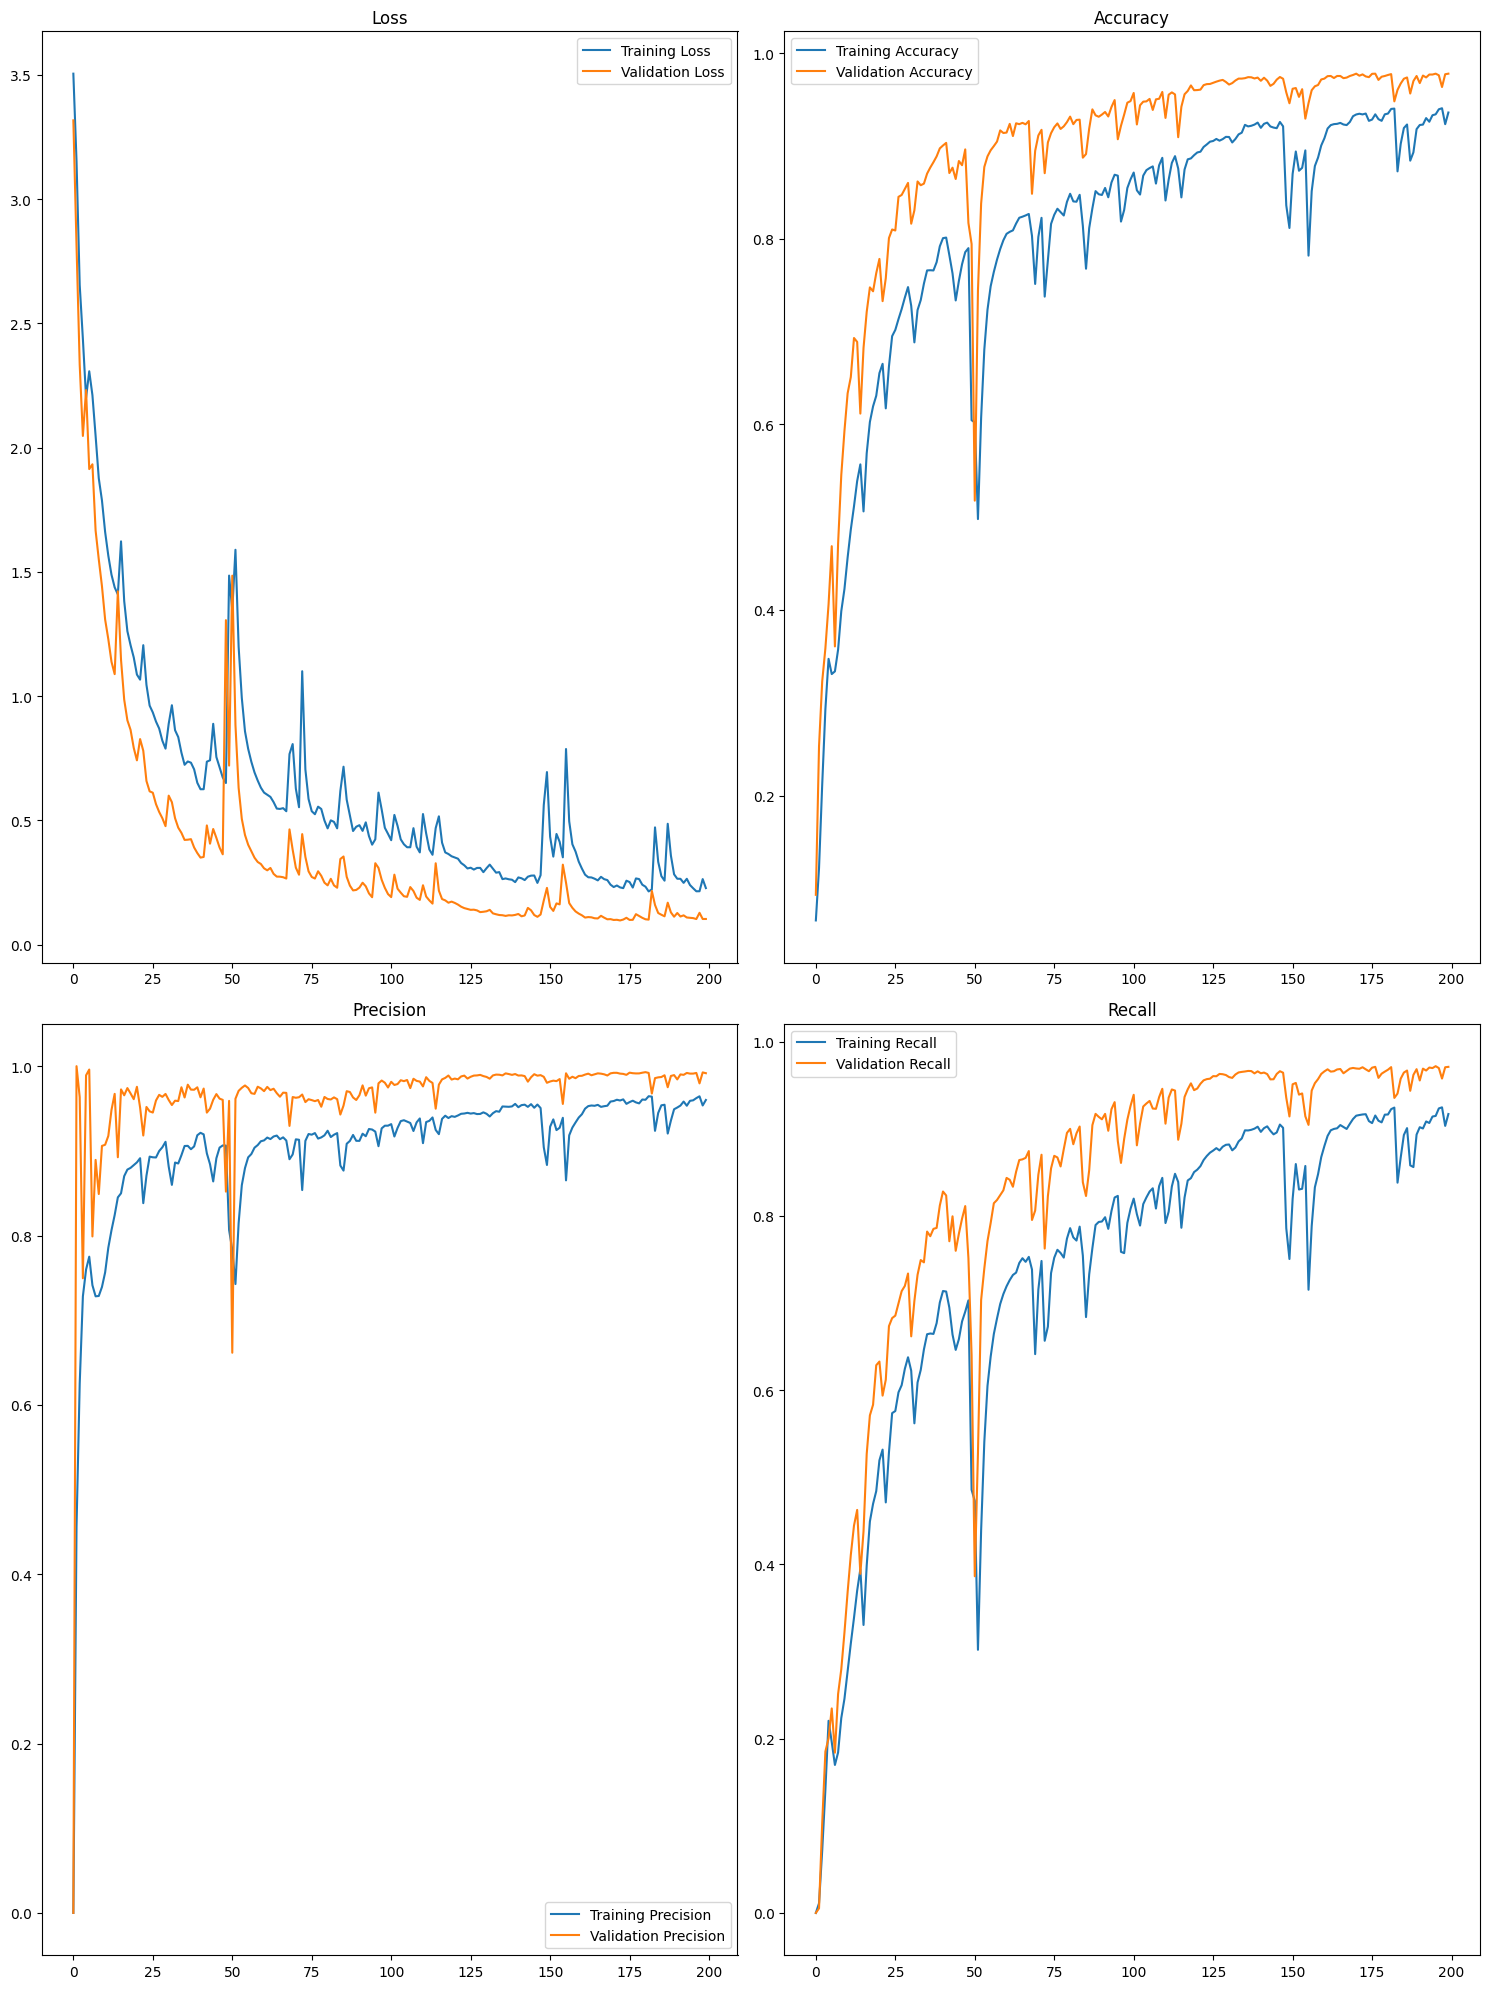
\includegraphics[width=\columnwidth]{images/ESED/ESD_training_400.png}
    \caption{L'andamento durante il training della RNN}
    \label{fig:train-400-esed}
\end{figure}
%
Quanto emerso è abbastanza incoraggiante \ref{fig:train-400-esed}: effettuato lo split del dataset in 70-10-20\% per il train-validation-test, si sono iniziati i lavori utilizzando una LSTM troppo complessa, che ha per un attimo ha abbassato il morale. 

Inizialmente si è immaginata come causa l'eccessivo numero di classi, andando ad arrivare a filtrare il numero di classi mantenendo solo quelle con più di 3.000 occorrenze; ci si è poi resi conto dei difetti di progettazione dell'architettura in merito al problema in questione, arrivando all'ottimo risultati con un dataset in cui vengono filtrate solo le classi con meno di 400 occorrenze, mantenendone in totale ben 37. 

L'andamento ora è regolare del training vola verso le migliori performance immaginabili, tracciando però anche un possibile spettro di una scarsa capacità di generalizzazione all'infuori del dataset; in ogni caso, con performance simili non vi sarebbe bisogno nemmeno di discutere ed effettuare il tuning del modello per capire se ottenere in output uno strumento recall vs precision oriented.
%
\begin{table}[h]
\begin{tabular}{lllll}
             & \textbf{precision} & \textbf{recall} & \textbf{f1-score} & \textbf{suport} \\
CWE-114      & 0.98               & 0.99            & 0.99              & 115             \\
CWE-119      & 0.99               & 1.00            & 0.99              & 236             \\
CWE-121      & 0.98               & 0.99            & 0.99              & 1002            \\
CWE-122      & 0.99               & 1.00            & 0.99              & 1191            \\
CWE-124      & 0.98               & 0.97            & 0.97              & 441             \\
CWE-126      & 0.98               & 0.87            & 0.92              & 349             \\
CWE-127      & 0.98               & 0.95            & 0.97              & 441             \\
CWE-134      & 0.99               & 0.99            & 0.99              & 587             \\
CWE-190      & 1.00               & 0.99            & 1.00              & 818             \\
CWE-191      & 0.98               & 0.98            & 0.98              & 635             \\
CWE-194      & 0.99               & 0.98            & 0.98              & 251             \\
CWE-195      & 0.99               & 0.95            & 0.97              & 251             \\
CWE-197      & 0.96               & 0.93            & 0.95              & 194             \\
CWE-23       & 1.00               & 1.00            & 1.00              & 480             \\
CWE-252      & 1.00               & 0.99            & 1.00              & 127             \\
CWE-253      & 1.00               & 1.00            & 1.00              & 137             \\
CWE-36       & 1.00               & 1.00            & 1.00              & 480             \\
CWE-369      & 0.99               & 0.88            & 0.93              & 195             \\
CWE-400      & 0.91               & 0.92            & 0.92              & 182             \\
CWE-401      & 0.99               & 0.98            & 0.99              & 355             \\
CWE-415      & 1.00               & 0.95            & 0.97              & 203             \\
CWE-416      & 0.94               & 0.98            & 0.96              & 103             \\
CWE-427      & 1.00               & 0.99            & 0.99              & 96              \\
CWE-457      & 0.97               & 0.98            & 0.98              & 193             \\
CWE-476      & 0.69               & 0.96            & 0.80              & 296             \\
CWE-563      & 1.00               & 1.00            & 1.00              & 103             \\
CWE-590      & 1.00               & 0.99            & 1.00              & 545             \\
CWE-606      & 0.99               & 0.98            & 0.98              & 98              \\
CWE-680      & 0.94               & 0.99            & 0.96              & 117             \\
CWE-690      & 1.00               & 1.00            & 1.00              & 192             \\
CWE-758      & 1.00               & 1.00            & 1.00              & 116             \\
CWE-761      & 0.96               & 0.95            & 0.96              & 123             \\
CWE-762      & 1.00               & 1.00            & 1.00              & 713             \\
CWE-78       & 1.00               & 0.98            & 0.99              & 1024            \\
CWE-789      & 1.00               & 0.94            & 0.97              & 215             \\
CWE-89       & 0.83               & 0.77            & 0.80              & 94              \\
CWE-90       & 0.93               & 0.98            & 0.95              & 96              \\
accuracy     &                    &                 & 0.98              & 12794           \\
macro avg    & 0.97               & 0.97            & 0.97              & 12794           \\
weighted avg & 0.98               & 0.98            & 0.98              & 12794          
\end{tabular}
\end{table}

Bisogna tuttavia ricordare che questo dataset è relativamente piccolo e che non contiene codice che non presenti vulnerabilità; ciononostante, si è riusciti a sottolineare le potenzialità di SARD nella bontà dei dati nella capacità di distinguere le diverse tipologie CWE in codice C/C++ tra loro.

\section{Analisi}

\textbf{In questa sezione si affrontano diverse questioni e dubbi sorti durante l'approfondimento in merito alle tecniche di deep learning applicate al contesto della sicurezza informatica.}

\subsection{Disponibilità dei dati}
Nell'approfondimento non sono stati utilizzati embedding pre-addestrati specifici su codice (e non) a causa delle limitate risorse hardware - il caricamento di questi causava facilmente il crash del runtime su Google Colab. In questo ambito non esiste attualmente il corrispettivo di quello che è \textit{ImageNet} per la classificazione di immagini, oppure il COCO per l'object detection. Anzi, come descritto nella sezione iniziale i dati sono abbastanza sparpagliati e mal supportati, e generalmente ogni organizzazione segue un proprio standard. L'enorme richiesta di dati da parte del Deep Learning richiede l'introduzione di standard e l'unione delle forze può essere il punto di svolta per questo ambito.
\textbf{La generazione di dataset sintetici} potrebbe essere un fronte interessante per aumentare la quantità di dati disponibili, ma risulta essere ancora un mondo delicato, oltre al fatto che non si potrebbe affermare che un codice sintetico generato da un codice vulnerabile sia a sua volta vulnerabile, richiedendo comunque un etichettamento, manuale o automatico che sia.

\subsection{Codice non vulnerabile certificato}
Lo sviluppo più interessante riguarderebbe, oltre a un'analisi più approfondita dello stato dell'arte odierna, il completamento del dataset costruito ESED con altrettanti esempi di codice considerabile come non-vulnerabile - in sostanza, un VDISC ma "affidabile". Alcuni dataset esistenti contengono riferimenti a repository GitHub dove è presente sia il codice con la vulnerabilità individuata che il codice con la vulnerabilità corretta. Tuttavia, chi può affermare che quest'ultimo non sia affetto da altre possibili vulnerabilità? Per questo motivo risulta logica il non usufruire di queste patch disponibili.

Una soluzione a ciò potrebbe essere essere il cambio di filosofia, selezionando un sottoinsieme di vulnerabilità su cui si hanno delle chance di individuazione, affermando che: \textbf{\textit{"il codice o contiene un possibile sottoinsieme di vulnerabilità oppure non le contiene"}}, eliminando il concetto di "non vulnerabile" (aka corretto). Ciò si sconterebbe comunque con la difficoltà dell'etichettamento su un grande quantitativo di dati, descritto nella sezione successiva.

\subsection{Etichettamento automatico}
Come effettuato per il dataset VDISC, per etichettare una grande quantità di dati serve incrociare i risultati tool di analisi - da quanto affermato nel paper, obbligatoriamente statica - esistenti attualmente. Questo è avvenuto sii nella ricerca citata più volte \cite{russell2018automatedvulnerabilitydetectionsource}, dove sono stati utilizzati solo tool di analisi statica \textit{flawfinder}, \textit{CCpcheck} e \textit{Clang}, i cui output tuttavia sono stati dovuti trattare da un tram di persone umane per creare una corrispondenza - non resa nota - tra output/CWE.

La potenzialità di questo processo è quello di unire in un unico strumento - un modello di deep learning - le potenzialità di più tool di analisi (statica).

\subsection{Sbilanciamento reale}

Come già citato, resta lecito il domandarsi se lo sbilanciamento dei dati verso il "non-vulnerabile" sia effettivamente un riflesso della realtà oppure no. La problematica di questo ambito è il duplice etichettamento intrinseco: per etichettare un codice come vulnerabile devo rilevare la vulnerabilità, ma anche per etichettare un codice come non vulnerabile devo certificarne la veridicità. Per risolvere ciò, si potrebbe concentrare gli sforzi su un sottoinsieme di vulnerabilità, come è stato fatto con alcuni tool di analisi statica, andando a considerare per esempio l'individuazione delle vulnerabilità difficili da rilevare con tool di analisi statica e dinamica - che però richiederebbero una certificazione manuale, cosa alquanto difficile in enormi quantità di dati.

\subsection{Explainability e prevedibilità}

Come sperimentato nelle diverse prove del dataset, le architetture CNN e RNN - non di certo le più moderne e capaci, ma valide per la leggerezza - sono abbastanza delicate nella costruzione dell'architettura, così come nella scelta dei parametri di tokenization, rispondendo molto diversamente al cambio di certe strutture senza compiere stravolgimenti. Se uniamo questa imprevedibilità al fatto che ci stiamo affidando a dei modelli matematici di cui non sappiamo comprendere il perché delle risposte, si potrebbe entrare nel mondo della filosofia e dell'analisi del pensiero umano, affermando che: \textit{"stiamo costruendo uno strumento imprevedibile dunque, in un certo senso, inaffidabile, per migliorare l'affidabilità"}. Non di certo le premesse migliori per parlare di "sicurezza".

\subsection{Framing effect}
\textit{Premessa: l'interpretazione è personale ed è assolutamente oggetto di discussione in mancanza di competenze, ma di un interesse, nell'ambito.}

Il bias cognitivo definito \textit{framing effect}; ragioniamo su questo esempio:
\begin{itemize}
    \item Un tool di analisi statica rileva 400 vulnerabilità su 1.000
    %
    \item Un modello di deep learning rileva generalmente il 40\% delle vulnerabilità
\end{itemize}
%
In termini positivi, la mente umana preferisce i "termini assoluti", \textit{sicuri}, anziché a quelli probabilistici. 

Perciò, di primo impatto, se si dovesse scegliere, in un progetto dove la sicurezza è un argomento importante, tra un tool di analisi statica basato su una matematica consolidata e con risposte più "prevedibili", assolute (anche se magari più limitate), rispetto a un modello di deep learning di cui, generalmente, noi stimiamo le performance (senza riuscire a spiegare il perché le riesca a raggiungere), ci porterebbe forse alla prima soluzione?

\section{Conclusioni}

L'analisi delle tecniche di deep learning applicate alla rilevazione delle vulnerabilità nel codice C/C++ ha messo in luce un panorama complesso, e, per quanto sperimentato, non del tutto promettente. I modelli di deep learning dimostrano comunque un potenziale nella capacità di individuazione tra le diverse vulnerabilità, superando alcuni limiti delle tecniche di analisi statica tradizionali. Tuttavia, la qualità del dataset utilizzato per l'addestramento risulta essere un fattore cruciale. La creazione dei dataset VDISC e ESED ha mostrato che l'affidabilità delle etichette e la rappresentatività dei dati influenzano direttamente l'accuratezza del modello.

L'uso di strumenti di analisi statica per l'etichettatura, pur utile, può trasferire errori e limitazioni nei dati, evidenziando la necessità di un controllo più accurato. L'elevata prevalenza di etichette non vulnerabili ha creato uno sbilanciamento nel dataset, suggerendo l'importanza di tecniche di bilanciamento per migliorare le prestazioni del modello.

In sintesi, le tecniche di deep learning offrono nuove possibilità significative per la sicurezza del software, ma il loro successo dipende dalla qualità dei dati e dalla capacità di affrontare le sfide inerenti alla creazione e alla gestione di dataset complessi. Per avanzare ulteriormente in questo campo, sarà essenziale continuare a migliorare i processi di raccolta ed etichettamento dei dati, sfruttando prettamente i tool di analisi statica esistenti. La strada da percorrere può essere promettente, ma richiede una maggiore unità nella comunità internazionale.

\bibliographystyle{./IEEEtran}
\bibliography{biblio}

\end{document}
